\documentclass[11pt,letterpaper]{article}
\usepackage[T1]{fontenc}
\usepackage[utf8]{inputenc}
\usepackage{lmodern}
\usepackage[letterpaper,margin=1in]{geometry}
\usepackage{amsmath,amssymb,amsfonts,mathtools,bm}
\usepackage{booktabs,array,multirow}
\usepackage{graphicx,tikz,pgfplots,pgfplotstable,xcolor}
\usetikzlibrary{arrows.meta,positioning,shapes.geometric}
\pgfplotsset{compat=1.18}
\usepackage{microtype,caption,fancyhdr,lastpage,enumitem}
\usepackage[numbers,sort&compress]{natbib}
\usepackage[colorlinks=true,linkcolor=blue,citecolor=blue,urlcolor=blue]{hyperref}
\setlength{\headheight}{14pt}
\emergencystretch=2em
\setlist{nosep,topsep=3pt}

% palette inspired by the COSC 750 paper style
\definecolor{prAmber}{HTML}{B7791F}
\definecolor{prBlue}{HTML}{2B6CB0}
\definecolor{prGreen}{HTML}{2F855A}
\definecolor{prPurple}{HTML}{6B46C1}
\definecolor{prGray}{HTML}{4A5568}

\pagestyle{fancy}\fancyhf{}
\lhead{\small\textsc{COSC 573 --- Naive Bayes Spam Filtering}}
\rhead{\small\textsc{Preprint}}
\cfoot{\small\thepage}
\renewcommand{\headrulewidth}{0.4pt}
\title{\vspace{-1.3em}\LARGE\bfseries Implementation and Experimental Evaluation\\of a Naive Bayes Spam Filtering System\\Using Python\vspace{.3em}}
\author{Nimi Kenanagha\\Department of Computer Science, Bowie State University\\\texttt{kenanaghan0131@students.bowiestate.edu}\\[.4em]{\small COSC 573 --- Artificial Intelligence \quad $\cdot$ \quad Fall 2026}}
\date{}

% CSV inputs for regenerable tables and figures
\pgfplotstableread[col sep=comma]{labeled_results.csv}\labeledtable
\pgfplotstableread[col sep=comma]{diagnostic_results.csv}\diagnostictable
\pgfplotstableread[col sep=comma]{word_ratios.csv}\ratiotable
\pgfplotstableread[col sep=comma]{figure_word_posteriors.csv}\wordchart
\pgfplotstableread[col sep=comma]{figure_repeat.csv}\repeatchart

\begin{document}
\maketitle\thispagestyle{fancy}
\begin{abstract}
Spam filtering is a probabilistic text-classification task in which individual tokens provide uncertain evidence about a message's class. This work implements a two-class multinomial Naive Bayes filter in Python from the supplied SpamHam educational starter package. The implementation uses 6,245 spam vocabulary entries (75,268 token occurrences) and 16,207 ham entries (290,673 token occurrences), equal class priors, a fixed $10^{-5}$ likelihood floor, and log-domain inference. We evaluate the two instructor-provided labeled messages and 11 additional controlled diagnostics that probe individual word signals, conflicting evidence, repetition, case and punctuation sensitivity, and numerical stability. Both prescribed tests pass: the supplied spam message yields a reported posterior of 1.0 (rounded to machine precision), while the ham example yields $3.641589521379177\times10^{-46}$. The diagnostic cases illustrate interpretable evidence accumulation and expose limitations in preprocessing and probability flooring. These results establish functionality on the supplied examples, not population-level accuracy or calibration. The paper presents explicit derivations, regenerable figures and tables, executable reproducibility steps, and bounded proposals for further evaluation.
\end{abstract}
\noindent\textbf{Keywords:} naive Bayes; spam detection; text classification; probabilistic reasoning; reproducible experiments; log-likelihood.

\section{Introduction}
Unsolicited email and other unwanted messages impose attention, security, and infrastructure costs. A spam filter maps a tokenized message $m=(w_1,\ldots,w_n)$ to a class $C\in\{S,H\}$, where $S$ denotes spam and $H$ legitimate (ham) content. Unlike a hand-coded keyword blacklist, a probabilistic model combines evidence across the message. Naive Bayes is especially suitable for a transparent programming exercise: its parameters can be estimated from word-frequency files and its decisions can be reconstructed mathematically \citep{russell2022,raschka2014}.

This project is a faithful implementation of the supplied \texttt{SpamHam.zip} assignment rather than an attempt to recreate the full Apache SpamAssassin system. SpamAssassin uses multiple filtering mechanisms; the assignment supplies preaggregated word counts with frequent stop-words and singleton counts removed \citep{assignment,spamassassin}. The two supplied messages have labels, whereas the additional diagnostic strings are constructed probes, not an independent labeled evaluation set.

\subsection{Research questions and contributions}
\noindent\textbf{RQ1:} Can a directly programmed word-frequency Naive Bayes filter pass the supplied labeled classification tests?\\
\textbf{RQ2:} How do word evidence, repetition, mixed evidence and unknown tokens affect posterior predictions?\\
\textbf{RQ3:} What limitations of the chosen likelihood floor and tokenizer are visible from controlled diagnostics?

The contributions are (i) a standard-library Python implementation in the supplied interface, (ii) numerical derivations tied to the data, (iii) reproducible tests and saved CSV summaries, and (iv) a critique that separates observed behavior from generalization claims.

\section{Related Work and Theoretical Context}
Russell and Norvig \citep{russell2022}, Chapter 12, introduce Bayes' rule and naive Bayes models as tractable inference under simplifying independence assumptions. Raschka \citep{raschka2014} discusses the link between probabilistic classification, feature representation and the naive assumption. Sahami et al. \citep{sahami1998} demonstrated the relevance of Bayesian modeling to junk-email filtering, including the practical importance of feature design and classification error costs. Apache SpamAssassin provides an example of a deployed multi-method spam-detection system \citep{spamassassin}. These sources motivate the model but do not establish that our two-example classroom test estimates real-world accuracy.

For this project, probabilities are estimated from \emph{token occurrence counts}, not document frequencies. This distinction makes a multinomial bag-of-words likelihood the natural model: repeating a word changes the evidence. The class counts do not identify the numbers of training messages and therefore do not justify empirical message-class priors.

\section{Data and Implementation}
\subsection{Provided data and example inputs}
\begin{table}[ht]
\centering\caption{Supplied corpus summaries computed from the two count files. The totals represent token occurrences, not message counts.}\label{tab:corpus}
\begin{tabular}{lrr}\toprule
Property & Spam & Ham\\\midrule
Unique listed words & 6,245 & 16,207\\
Total token occurrences & 75,268 & 290,673\\
Provided example & \texttt{spamesim.txt} & \texttt{hamesim.txt}\\
Whitespace-separated example tokens & 140 & 232\\\bottomrule
\end{tabular}
\end{table}
The template's \texttt{get\_occurrences} reads \texttt{count word} pairs into Python dictionaries. The \texttt{get\_words} routine tokenizes test files with \texttt{split()}, retaining punctuation and capitalization. The completed \texttt{SpamHam.evaluate(words)} method returns a floating-point posterior probability, as required by \texttt{test/test\_main.py}. Only the missing evaluation method was necessary for the core assignment; the auxiliary experiment script adds diagnostics and CSV exports.

\subsection{Reproducible processing flow}
\begin{figure}[ht]
\centering
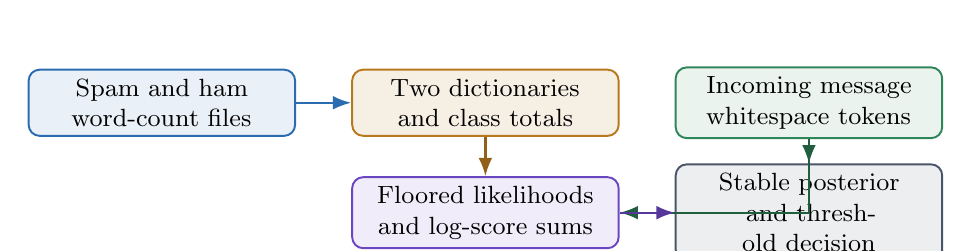
\begin{tikzpicture}[node distance=5mm and 7mm,>=Latex, every node/.style={font=\small}, mybox/.style={draw,rounded corners,align=center,minimum height=8mm,text width=3.15cm,line width=.7pt}]
\node[mybox,fill=prBlue!10,draw=prBlue] (counts) {Spam and ham\\word-count files};
\node[mybox,right=of counts,fill=prAmber!12,draw=prAmber] (dict) {Two dictionaries\\and class totals};
\node[mybox,right=of dict,fill=prGreen!10,draw=prGreen] (message) {Incoming message\\whitespace tokens};
\node[mybox,below=of dict,fill=prPurple!10,draw=prPurple] (score) {Floored likelihoods\\and log-score sums};
\node[mybox,right=of score,fill=prGray!10,draw=prGray] (post) {Stable posterior\\and threshold decision};
\draw[->,thick,prBlue] (counts)--(dict);
\draw[->,thick,prAmber!80!black] (dict)--(score);
\draw[->,thick,prGreen!70!black] (message)--(post);
\draw[->,thick,prGreen!70!black] (message.south) |- (score.east);
\draw[->,thick,prPurple!80!black] (score)--(post);
\end{tikzpicture}
\caption{Implemented inference pipeline. Training counts are supplied; the program does not retrain from individual raw messages. Diagram authored for this manuscript as vector graphics.}\label{fig:pipeline}
\end{figure}

\section{Mathematical Methodology}
\subsection{Bayes' rule and class priors}
For message $m$, Bayes' rule gives
\begin{equation}\label{eq:bayes}
P(S\mid m)=\frac{P(m\mid S)P(S)}{P(m\mid S)P(S)+P(m\mid H)P(H)}.
\end{equation}
Because class-level message counts are unavailable, the implementation specifies $P(S)=P(H)=\tfrac12$. This is a transparent modeling assumption, not an observed deployment prevalence. A posterior greater than $0.5$ is labeled spam; less than $0.5$, ham; exactly $0.5$, a tie for the experiment report.

\subsection{Class-conditional word estimates}
Let $c_C(w)$ be the occurrence count of word $w$ in class $C$ and $N_C=\sum_{w}c_C(w)$. The raw relative-frequency estimator is
\begin{equation}\label{eq:likelihood}
\widehat P(w\mid C)=\frac{c_C(w)}{N_C},\quad C\in\{S,H\}.
\end{equation}
For \texttt{free} the supplied counts are 624 (spam) and 438 (ham), giving
\begin{align}\label{eq:free}
\widehat P(\texttt{free}\mid S)&=624/75268=0.00829038,\\
\widehat P(\texttt{free}\mid H)&=438/290673=0.00150685.
\end{align}
The template defines $\epsilon=10^{-5}$. The implementation uses
\begin{equation}\label{eq:floor}
q_C(w)=\max\{\widehat P(w\mid C),\epsilon\}.
\end{equation}
This floor prevents undefined $\log 0$, but is \emph{not} the same as additive (Laplace/Lidstone) smoothing: it may alter known rare-word probabilities and the resulting $q_C$ values need not sum to one over a vocabulary.

\subsection{Multinomial assumption and log-domain inference}
Assuming token occurrences are conditionally independent given the class, and ignoring a class-independent multinomial coefficient, the class score for message $m$ is proportional to
\begin{equation}\label{eq:product}
L_C(m)=P(C)\prod_{i=1}^{n}q_C(w_i).
\end{equation}
Repeated terms appear once per occurrence. Multiplying many probabilities directly underflows for long messages, so compute
\begin{equation}\label{eq:logscore}
\ell_C=\log P(C)+\sum_{i=1}^{n}\log q_C(w_i).
\end{equation}
Define the \emph{log odds favoring ham} as $\Delta=\ell_H-\ell_S$. Then
\begin{equation}\label{eq:sigmoid}
P(S\mid m)=\frac{1}{1+\exp(\Delta)}.
\end{equation}
For $\Delta\ge0$, the code instead evaluates $e^{-\Delta}/(1+e^{-\Delta})$; for $\Delta<0$, it evaluates $1/(1+e^{\Delta})$. This branch avoids overflow and keeps the posterior in $[0,1]$.

\subsection{Worked single-word example}
For a message consisting only of the token \texttt{free},
\begin{equation}\label{eq:singlefree}
P(S\mid \texttt{free})=
\frac{q_S(\texttt{free})P(S)}{q_S(\texttt{free})P(S)+q_H(\texttt{free})P(H)}.
\end{equation}
Using the values in Eq.~\eqref{eq:free} and equal priors,
\begin{equation}\label{eq:singlefree2}
P(S\mid \texttt{free})=
\frac{0.00829038\cdot 0.5}{0.00829038\cdot 0.5+0.00150685\cdot 0.5}
\approx 0.846196.
\end{equation}
The resulting $84.62\%$ is the posterior for that one-token input \emph{under the specified model}, not the unconditional probability that any message containing the word is spam. For $k$ copies of the same token, posterior odds scale as $\{q_S(w)/q_H(w)\}^{k}$, explaining why repeated \texttt{free} tokens strengthen the spam prediction.

\section{Experiment Protocol and Reproducibility}
Experiments use the exact supplied dictionaries and do not alter the classifier parameters. The complete protocol comprises two labeled example messages and 11 hand-constructed diagnostic cases. The latter test the mapping from inputs to posterior probabilities; they are not statistically representative of authentic messages. The auxiliary script \texttt{run\_experiments.py} records cases, token counts, exact returned probabilities, predicted labels and any provided ground-truth labels in \texttt{experiment\_results/classifications.csv}; a second CSV records selected class counts and raw/floored word likelihoods.

All experimental figures and result tables in this manuscript are \emph{regenerable} from the CSV files bundled in the source package. The Overleaf source includes the raw experimental CSVs (\texttt{classifications.csv} and \texttt{word\_probabilities.csv}) together with small derived CSVs for plot-ready summaries. The PDF figures are therefore rebuildable without re-running model training. Recompiling the manuscript reproduces the visualizations from saved outputs; this is not independent verification of the original experiments. The two labeled messages are the only cases with supplied ground truth (both instructor tests passed); the other eleven are controlled diagnostics, not an accuracy estimate.

\noindent\textbf{Reproduction commands} (run in the repository's \texttt{SpamHam} subfolder):
\begin{verbatim}
python3 src/main.py
python3 run_experiments.py
python3 -m testrunner
\end{verbatim}
The student's local Windows execution of the instructor-supplied tests reported \texttt{Ran 2 tests in 0.003s --- OK}. This is a test-suite execution time, \emph{not} a benchmark of prediction latency; timing includes test-runner overhead. The GitHub repository is \url{https://github.com/Tamaranimi/COSC573-NaiveBayes-SpamFilter}.

\section{Experimental Results}
\subsection{Instructor-labeled example messages}
\begin{table}[ht]
\centering
\caption{Observed instructor-supplied labeled tests. The displayed spam probability of 1.0 is affected by floating-point rounding; it is not logical certainty. Table regenerates from \texttt{labeled\_results.csv}.}\label{tab:labeled}
\pgfplotstabletypeset[
col sep=comma,
string type,
columns={input_file,tokens,posterior,predicted_label,status},
columns/input_file/.style={column name=Input file,column type=l},
columns/tokens/.style={column name=Tokens,column type=r},
columns/posterior/.style={column name=$P(S\mid m)$,column type=r},
columns/predicted_label/.style={column name=Predicted,column type=l},
columns/status/.style={column name=Status,column type=l},
every head row/.style={before row=\toprule,after row=\midrule},
every last row/.style={after row=\bottomrule}
]{\labeledtable}
\end{table}
Both instructor tests passed (2/2). This success supports correctness on these supplied examples and compliance with the public test interface only. With $n=2$ labeled cases there is no sound basis for claims about unseen-population precision, recall, F1, false-positive rate or calibrated probability quality.

\subsection{Diagnostic inputs}
\begin{table}[ht]
\centering
\caption{Observed controlled diagnostics, regenerated from \texttt{diagnostic\_results.csv}. Labels here are decisions, not independently verified ground truth.}\label{tab:diagnostics}
\scriptsize
\pgfplotstabletypeset[
col sep=comma,
string type,
columns={display_case,tokens,posterior,decision},
columns/display_case/.style={column name=Input/case,column type=p{5.1cm}},
columns/tokens/.style={column name=Tokens,column type=r},
columns/posterior/.style={column name=$P(S\mid m)$,column type=r},
columns/decision/.style={column name=Decision,column type=l},
every head row/.style={before row=\toprule,after row=\midrule},
every last row/.style={after row=\bottomrule}
]{\diagnostictable}
\end{table}

\begin{figure}[ht]
\centering
\begin{tikzpicture}
\begin{axis}[
xbar,
width=.88\linewidth,
height=5.3cm,
xmin=0,xmax=100,
bar width=9pt,
xlabel={Posterior probability of spam (\%)},
symbolic y coords={listinfo,linux,free,money},
ytick=data,
nodes near coords,
nodes near coords align={horizontal},
every node near coord/.append style={font=\scriptsize},
axis x line*=bottom,
axis y line*=left,
grid=major,
grid style={gray!15},
enlarge y limits=.18]
\addplot[fill=prBlue!55,draw=prBlue!90!black] table[x=spam_percent,y=word,col sep=comma] {figure_word_posteriors.csv};
\end{axis}
\end{tikzpicture}
\caption{Observed posterior spam probabilities for four selected one-token inputs. The chart regenerates from \texttt{figure\_word\_posteriors.csv}. It describes conditional responses to constructed inputs, not classification accuracy across labeled messages.}\label{fig:words}
\end{figure}

\subsection{Effect of combining and repeating evidence}
\begin{figure}[ht]
\centering
\begin{tikzpicture}
\begin{axis}[
ybar,
width=.85\linewidth,
height=5.0cm,
ymin=0,ymax=100,
bar width=19pt,
ylabel={Posterior spam probability (\%)},
symbolic x coords={free,free x5,free+linux},
xtick=data,
nodes near coords,
nodes near coords align={vertical},
every node near coord/.append style={font=\scriptsize},
grid=major,
grid style={gray!15}]
\addplot[fill=prAmber!60,draw=prAmber!90!black] table[x=case_label,y=spam_percent,col sep=comma] {figure_repeat.csv};
\end{axis}
\end{tikzpicture}
\caption{Contrasting controlled cases: adding \texttt{linux} moderates the spam evidence from \texttt{free}, while repeating \texttt{free} five times strengthens it. The plot regenerates from \texttt{figure\_repeat.csv}.}\label{fig:repeat}
\end{figure}

\begin{table}[ht]
\centering
\caption{Illustrative token counts and likelihood ratios, regenerated from \texttt{word\_ratios.csv}. Ratios are based on raw likelihoods where they exceed the fixed floor.}\label{tab:ratios}
\pgfplotstabletypeset[
col sep=comma,
string type,
columns={token,spam_count,ham_count,q_spam,ratio},
columns/token/.style={column name=Token,column type=l},
columns/spam_count/.style={column name=Spam count,column type=r},
columns/ham_count/.style={column name=Ham count,column type=r},
columns/q_spam/.style={column name=$q_S(w)$,column type=r},
columns/ratio/.style={column name=$q_S(w)/q_H(w)$,column type=r},
every head row/.style={before row=\toprule,after row=\midrule},
every last row/.style={after row=\bottomrule}
]{\ratiotable}
\end{table}
The relative-frequency ratios explain the single-token posteriors: $P(S\mid w)=r/(1+r)$ for $r=q_S(w)/q_H(w)$ with equal priors. Figure~\ref{fig:repeat} and Table~\ref{tab:diagnostics} demonstrate how evidence accumulates with repetition. Two novel variants, \texttt{Free} and \texttt{free!}, both return the neutral 0.5 score under exact token matching, exposing case and punctuation sensitivity. Long repetition of an unseen token also returns 0.5 without numerical failure; this is a \emph{stability} test rather than a speed test.

\section{Discussion and Threats to Validity}
\subsection{What the experiments support}
RQ1 is answered positively for the provided interface: the classifier produces the expected extreme spam and ham posteriors, and both instructor tests pass. For RQ2, the individual-word and combined-word results exhibit the direction predicted by likelihood ratios; repeating \texttt{free} compounds evidence in the multinomial model. For RQ3, case- and punctuation-sensitive tokens cause exact-match failures, and a common floor yields a neutral score for evidence unseen in both classes. The log-domain computation remains finite for the 1,000-token unseen-string check.

\subsection{Interpretability versus calibrated probability}
Scores are interpretable as outputs of the specified probabilistic model, but not necessarily calibrated probabilities for incoming mail. Equal class priors may not match operational spam prevalence. The independence assumption is false for many collocations and repeated structures. The fixed floor changes the likelihood family, particularly for rare terms; no calibration analysis or deployment sampling was performed. A reported 1.0 is a machine-precision representation of overwhelming evidence, not proof that the message \emph{cannot} be ham.

\subsection{Internal, external and construct validity}
The labeled evaluation comprises only two instructor-selected examples, and both may be easier than naturally occurring ambiguous mail. The 11 constructed diagnostics were chosen for mechanism inspection, not representative sampling. Source counts were preprocessed by upstream authors; the original message-level training data, message priors and preprocessing decisions are unavailable. Consequently, dataset leakage, temporal drift, false-positive harms and subgroup effects cannot be assessed. No precision/recall/confusion matrix is reported because these metrics would misleadingly treat controlled unlabeled cases as ground truth.

\section{Challenges, Improvements and Future Work}
\begin{enumerate}[leftmargin=*]
\item \textbf{Preprocessing consistency:} lowercase and tokenize both training and evaluation data consistently, with careful treatment of URLs, numbers, punctuation and Unicode. Changing only inference tokenization would create a train/test mismatch.
\item \textbf{Principled smoothing:} compare the current fixed floor with normalized additive smoothing $P_\alpha(w\mid C)=(c_C(w)+\alpha)/(N_C+\alpha |V|)$, explicitly defining the vocabulary $V$ and out-of-vocabulary policy. This is proposed, not implemented in the current tests.
\item \textbf{Class priors and decision costs:} estimate priors from message counts or vary them in a prespecified sensitivity analysis. If false positives are more costly, use a threshold informed by expected costs rather than assuming 0.5 is operationally optimal.
\item \textbf{Representative evaluation:} acquire a licensed independent set of labeled emails, preserve train/test separation, and report class-conditional confusion counts with precision, recall, F1, and uncertainty intervals. Evaluate ambiguous borderline messages and temporal changes.
\item \textbf{Efficiency and reproducibility:} cache class totals instead of summing them on every evaluation; include a fixed environment specification, automated boundary tests, and a license/provenance audit for source corpora.
\end{enumerate}

\section{Conclusion}
The project delivers a directly programmed Naive Bayes spam filter using supplied SpamHam word counts and a stable log-domain posterior computation. The two labeled assignment examples are classified correctly, and the instructor's two local tests pass. Eleven diagnostic inputs provide interpretable evidence concerning word likelihood ratios, repetition, mixed evidence, unknown words and tokenization limitations. The result is a reproducible educational implementation, not an externally validated production spam filter. Expanded independently labeled evaluation and principled smoothing are the key next steps.

\begin{thebibliography}{9}
\bibitem{russell2022} S. Russell and P. Norvig, \emph{Artificial Intelligence: A Modern Approach}, 4th ed., Global ed. Pearson, 2022. Ch.~12, Secs.~12.5--12.6.
\bibitem{raschka2014} S. Raschka, \emph{Naive Bayes and Text Classification I: Introduction and Theory}, arXiv:1410.5329, 2014 (subsequent revisions). \url{https://arxiv.org/abs/1410.5329}.
\bibitem{sahami1998} M. Sahami, S. Dumais, D. Heckerman, and E. Horvitz, ``A Bayesian approach to filtering junk e-mail,'' \emph{AAAI Workshop on Learning for Text Categorization}, 1998. \url{https://cdn.aaai.org/Workshops/1998/WS-98-05/WS98-05-009.pdf}.
\bibitem{assignment} \emph{Introduction to AI}, ``Naive Bayes spam filter'' assignment and \texttt{SpamHam.zip} starter package. \url{https://materiaalit.github.io/intro-to-ai/files/tests/SpamHam.zip}.
\bibitem{spamassassin} Apache Software Foundation, ``Apache SpamAssassin.'' \url{https://spamassassin.apache.org/}.
\end{thebibliography}
\end{document}
